\documentclass{article}
\usepackage{amsmath}
\usepackage{graphicx}
\usepackage{tikz}

\begin{document}

\begin{center}
    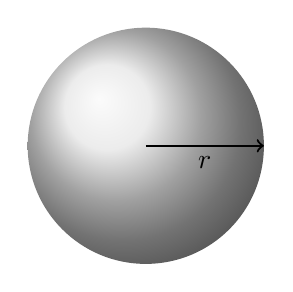
\begin{tikzpicture}
        % Draw the sphere with even lighter shading (light gray)
        \shade[ball color = gray!20] (0,0) circle (1.5);  % sphere shape
        
        % Draw the radius with one arrow, bold line
        \draw[thick,->] (0,0) -- (1.5,0) node[midway,below] {$r$};  % radius
    \end{tikzpicture}

    \hspace{2cm}  % Spacing between diagram and equations

    \begin{minipage}{3cm}
        \[
        A = 4\pi r^2
        \]
        \[
        V = \frac{4}{3} \pi r^3
        \]
    \end{minipage}

    \vspace{1cm}

    \textbf{Sphere}
\end{center}

\end{document}
